\section{Electropneumatic Implementation}


\subsection{Methodology}

The physical behaviour 
Several steps were taken in the implementation of the pneumatic system in order to facilitate

The top level of the Simulink model is shown in \ref{fig:pneumatics_top_level}: A PID controller block is used with closed-loop feedback, and the response to a fixed step input is displayed on the scope block.

In modelling the electropneumatic system, 3 subsystems were identified and modelled independently:

\begin{enumerate}
  \item the PWM generator;
  \item the solenoid valves;
  \item and the single-acting spring-return cylinder.
\end{enumerate}

\begin{figure}[h]
\centering
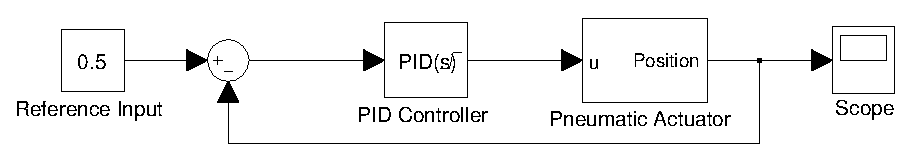
\includegraphics[scale=1]{implementation/figures/pneumatic_modelling1.eps}
\caption{Top-level electropneumatic model for simulation in Simulink.}
\label{fig:pneumatics_top_level}
\end{figure}

\paragraph{PWM Generator}

The PWM generator in Simulink was built using the instantaneous model presented by \citet{valve_models} which compares a generated saw-tooth signal, $V_{saw}$ with a period $T_{saw}$, with the input signal $V_{in}$ to obtain the pulse-width-modulated signal $U$:

%\begin{equation}
%U\left(t\right) = 
%\begin{cases}
%1 & V_{in}\left(t\right) \geq V_{saw}\left(t\right) \\
%0 & V_{in}\left(t\right) < \left(t\right)
%\end{cases}
%\end{equation}

               voltage saw-tooth signal Vd with period Tp the PWM signal U(t) can be expressed as
and amplitude Vp.


\begin{figure}[h]
\centering
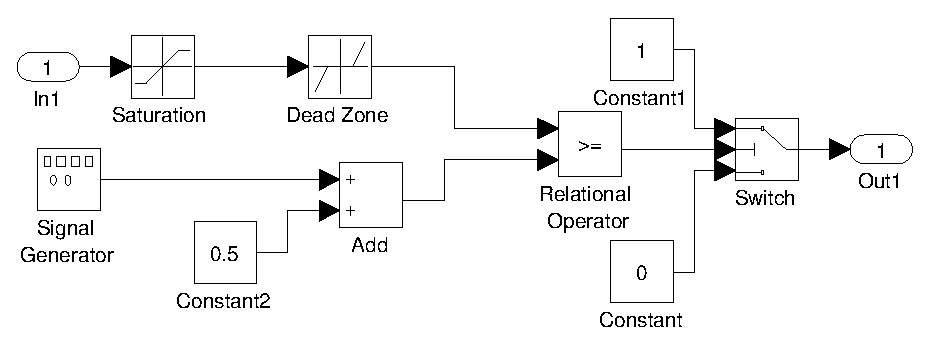
\includegraphics[scale=1]{implementation/figures/pneumatic_modelling2.eps}
\caption{Simulink PWM Generator model.}
\label{fig:pneumatics_pwm}
\end{figure}


\subsection{Solenoid Valves}


\subsection{Pneumatic Actuators}


\subsection{Positional Feedback Sensors}


\subsection{Mechanical Linkage}
